\documentclass[10pt, conference]{IEEEtran}

\newcommand{\ignore}[1]{}

% *** GRAPHICS RELATED PACKAGES ***
\usepackage[pdftex]{graphicx}
\usepackage{xcolor}
\usepackage{caption} %needed to make captions on figure* centered
\graphicspath{{./figures/}}
\DeclareGraphicsExtensions{.pdf,.png}
\usepackage[]{hyperref}

\usepackage[linesnumbered, ruled, vlined]{algorithm2e}

% correct bad hyphenation here
\hyphenation{Tele-operable}





\begin{document}
%
% paper title
\title{STOIC: Serverless Teleoperable Hybrid Cloud for Machine Learning Applications on Edge Device}


\author{\IEEEauthorblockN{Michael Zhang, Chandra Krintz, Rich Wolski}
\IEEEauthorblockA{Dept. of Computer Science \\
University of California, Santa Barbara\\
\{lebo, ckrintz, rich, mock\}@cs.ucsb.edu}
}
Markus' email: mock@haw-landshut.de
\author{\IEEEauthorblockN{Omitted for Blind Review}%\\
\IEEEauthorblockA{Blind Review \\
Blind Review\\
\{blind\}@blind.blind.blind}
}

% conference papers do not typically use \thanks and this command
% is locked out in conference mode. If really needed, such as for
% the acknowledgment of grants, issue a \IEEEoverridecommandlockouts
% after \documentclass

% for over three affiliations, or if they all won't fit within the width
% of the page, use this alternative format:
% 
%\author{\IEEEauthorblockN{Michael Shell\IEEEauthorrefmark{1},
%Homer Simpson\IEEEauthorrefmark{2},
%James Kirk\IEEEauthorrefmark{3}, 
%Montgomery Scott\IEEEauthorrefmark{3} and
%Eldon Tyrell\IEEEauthorrefmark{4}}
%\IEEEauthorblockA{\IEEEauthorrefmark{1}School of Electrical and Computer Engineering\\
%Georgia Institute of Technology,
%Atlanta, Georgia 30332--0250\\ Email: see http://www.michaelshell.org/contact.html}
%\IEEEauthorblockA{\IEEEauthorrefmark{2}Twentieth Century Fox, Springfield, USA\\
%Email: homer@thesimpsons.com}
%\IEEEauthorblockA{\IEEEauthorrefmark{3}Starfleet Academy, San Francisco, California 96678-2391\\
%Telephone: (800) 555--1212, Fax: (888) 555--1212}
%\IEEEauthorblockA{\IEEEauthorrefmark{4}Tyrell Inc., 123 Replicant Street, Los Angeles, California 90210--4321}}









% make the title area
\maketitle


\begin{abstract}
\label{sec:abstract}
Serverless computing emerges as a promising execution framework on the cloud for machine learning applications, considering the flexibility and elasticity it offers. However, the imbalance of computing resources between edge and public cloud dampens the availability and efficiency of serverless architecture, and consumes extraneous energy and costs from end users. 

The goal of our work is to bridge this gap by intelligently deploying tasks and making accelerator(e.g. GPU) serve edge devices in a robust and fault-tolerant fashion on serverless architecture. To enable this, we developed an open source cloud system called STOIC (Serverless TeleOperable HybrId Cloud), which leverages accelerators as a serverless service and schedules machine learning tasks across hybrid cloud system. Through our evaluation, STOIC largely outperforms single-runtime systems on real-world applications for IoT device and edge cloud. In this paper, we present the design and implementation of STOIC, along with the empirical evaluation of its efficacy and performance for machine learning applications.
\end{abstract}

\begin{IEEEkeywords}
Serverless computing; Model optimization; Hyperparameter tuning
\end{IEEEkeywords}


% For peer review papers, you can put extra information on the cover
% page as needed:
% \ifCLASSOPTIONpeerreview
% \begin{center} \bfseries EDICS Category: 3-BBND \end{center}
% \fi
%
% For peerreview papers, this IEEEtran command inserts a page break and
% creates the second title. It will be ignored for other modes.
\IEEEpeerreviewmaketitle



\section{Introduction}
\label{sec:intro}
Upon the recent shift of application architectures from monolithic to containers and microservices, serverless computing has risen as a promising cloud provider offering where event-driven functions compose all applications and services. It represents a revolutionary programming and deployment paradigm known as Function as a Service (FaaS). Using serverless model, developers can easily build up applications in a cloud without concerning server provisioning at the infrastructure level. Programmers usually write those functions in high-level languages and triggered by events either from external sources or, more often, internal cloud services. Thus, serverless architecture allows the application to distribute across the cloud by providing function-level abstraction.

Moreover, this function-level abstraction does not only abstract away the infrastructure management work from developers, but also, more importantly, provides more fine-grained computational resource isolation and usage, meaning each serverless function can autoscale independently based on the scale of incoming events. Providing such elasticity effectively avoids the single point failure and bottleneck service in a data-intensive application. From this perspective, serverless architecture is an ideal system for machine learning applications, especially for online training~\cite{ref:online} and model serving, because they usually transfer and handle a large amount of data, but the volume of each batch is uncertain and highly volatile depending on the data generated in that period. The flexibility that serverless functions deliver address such issue via the event-driven mechanism. 

To enable such an event-driven system, one concerning situation is that those machine learning applications usually evolve heterogeneous IoT devices, ranging from temperature sensors to mobile phones to autonomous drones, which are the primary data sources in the physical world. If the applications execute, at least partially, on the edge cloud, it could save lengthy round-trip time of transmitting data and make the application infinitely close to real-time. Such demand motivates us and we explore the effectiveness and efficiency of executing machine learning applications on the edge cloud in this work. 

An immediate difficulty we face is the scarcity of computational resources on edge cloud relative to high-demanding machine learning applications. In addition, no cloud provider offers serverless functions that leverage accelerators like GPU. In our work, we construct a hybrid cloud system that enables serverless function to utilize GPU, which substantially accelerates the execution of machine learning applications. We consider it as one of the key contributions of our research.

\begin{figure}
    \centering
    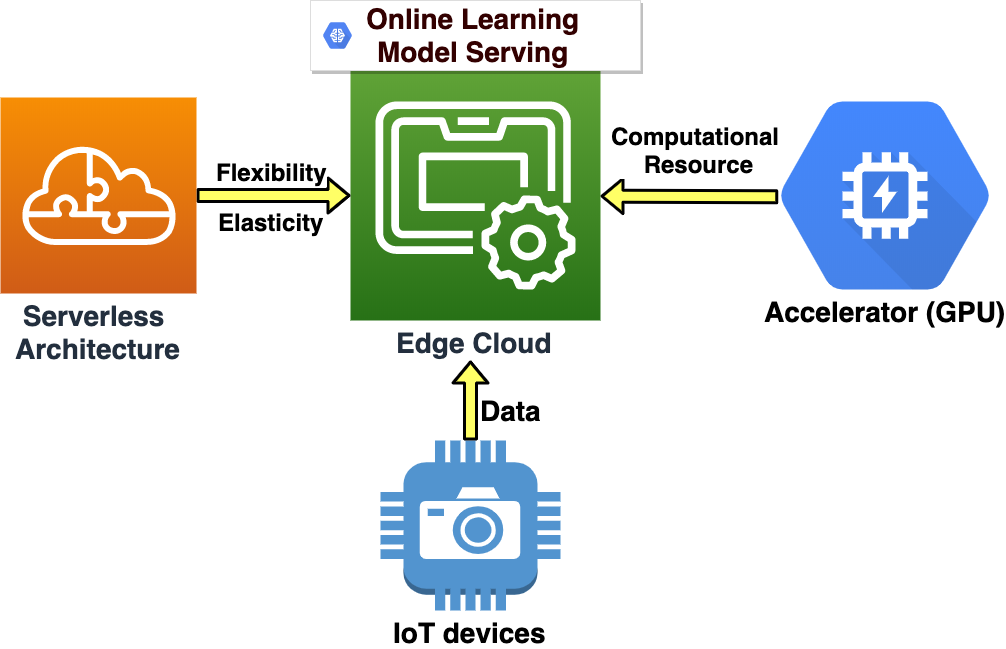
\includegraphics[scale=0.25]{figures/edge}
    \caption{\textbf{The Design Principle of STOIC}}
    \label{fig:edge}
\end{figure}

Figure~\ref{fig:edge} illustrates the design principles of our proposed system, STOIC (Serverless TeleOperable Hybrid Cloud). In our design, three underpinnings support the center edge cloud: IoT devices stream data in batches for training and inference; serverless architecture provides flexibility and elasticity to handle auto-scaling and unbalanced data payload; the accelerator offers an additional computational resource for extra large dataset and compute-intensive machine learning applications. In this paper, we discuss the design and implementation of this architecture, investigate the efficacy and  empirically evaluate its performance. We found STOIC reduces total response time, ranging from 6.48\% to 32.05\%, compared with four single runtimes. Finally, we show both related and future work and conclude.


%\section{Background}
%\label{sec:background}
%\input{background}

\section{Seneca}
\label{sec:seneca}
\input{Seneca}

\section{Evaluation}
\label{sec:eval}
In this section, we empirically evaluate STOIC's performance on executing machine learning applications, in contrast to single-runtime systems. We first outline the machine learning application benchmark that we consider, followed by our test on the application efficacy. Then an empirical experiment and its result are presented.

\subsection{Benchmark Application and Dataset}

We benchmark STOIC using an image processing application that classifies animal images from a wildlife monitoring system called ``Where's The Bear" (WTB)~\cite{ref:wtb}. ``Where's The Bear" is an end-to-end distributed data acquisition and analytics system that implements an IoT architecture and edge cloud. Our application inferences streaming photos taken by wildly deployed camera traps in Sedgwick Natural Reserve using a convolutional neural network (CNN)~\cite{ref:cnn} model trained by labeled images from the WTB dataset. Technically, it employs Tensorflow and Scikit-learn~\cite{ref:scikit} machine learning frameworks to perform the image classification.  

 In total, there are five classes that we consider in the CNN model training: Bird, Fox, Rodent, Human and Empty. Since the volume of classes are unbalanced due to different occurring frequency of animals, we up-sample the minority classes (e.g. fox) by Keras ImageDataGenerator~\cite{ref:keras} to ensure the classification model is not biased. Every image in the WTB dataset is resized to $1920 \times 1080$, and for each class, the dataset contains 251 images used to train CNN model. Once the model is trained, the application caches this model in hdf5 format and store it at both edge cloud disk storage and a shared volume in Ceph file system at Nautilus cloud. 

\subsection{Application Efficacy}

\begin{table}[t] \centering 
\scriptsize
\resizebox{\columnwidth}{!}{
\begin{tabular}{|c|c|c|c|c|} 
\hline
& \textbf{Mean $T_r$ (sec)} & \textbf{Stdev. $T_r$ (sec)} & \textbf{Mean $T_p$ (sec)} & \textbf{Stdev. $T_p$ (sec)}\\
\hline
edge & 108.88 & 1.65 & 108.88 & 1.65 \\
\hline
cpu & 100.0 & 4.93 & 86.99 & 4.92 \\
\hline
gpu1 & 98.90 & 4.03 & 50.65 & 4.05 \\
\hline
gpu2 & 106.29 & 5.53 & 39.21 & 5.55\\
\hline
\textbf{STOIC} & \textbf{97.73} & \textbf{3.13} & \textbf{50.49} & \textbf{3.11} \\
\hline
\end{tabular}
}
\caption{\textbf{Mean and stdev of total response time~($T_r$) and processing time~($T_p$) of 40-image batch}: STOIC schedules tasks onto the runtime (\textit{gpu1}) that has the least total response time~($T_r$).
\label{tab:validation}}
\end{table}

We first test the efficacy of STOIC by processing an image batch of fixed size at four runtimes individually and then compare with STOIC. To make the result reliable, we again conduct the experiment 10 times and list the mean and standard deviation of total response time~($T_r$) and processing time~($T_p$) in Table~\ref{tab:validation}. We can observe from Table~\ref{tab:validation} that STOIC schedules 40-image batch to \textit{gpu1} runtime, based on its prediction that  \textit{gpu1} would have the least total response time~($T_r$). One important observation is that \textit{gpu2} runtime has even lower processing time~($T_p$) than \textit{gpu1}, but STOIC disregard \textit{gpu2} in this scenario, because its gain in processing time~($T_p$) does not compensate its lengthy deployment time~($T_d$) on Nautilus cloud.

\begin{figure}[t] \centering 
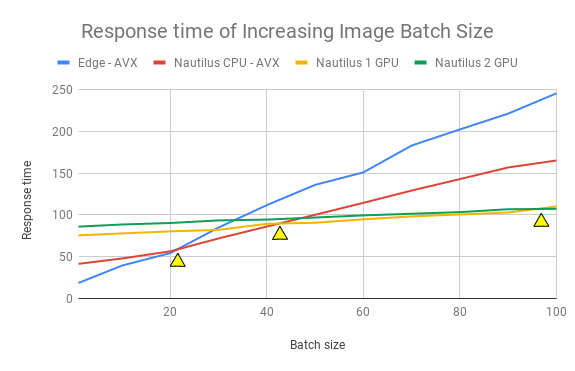
\includegraphics[scale=0.32]{response-time}
\caption{\textbf{Total Response Time~($T_r$) of image batches of growing sizes}: The x-axis represents batch size, while y-axis is the total response time~($T_r$). STOIC, which is depicted in blue dashed line, schedules the task on the runtime with the least total response time.  
\label{fig:response-time}}
\end{figure}

Additionally, we test STOIC by processing a series of image batches of growing sizes both on four runtimes and STOIC. The progressive response times are depicted in Figure~\ref{fig:response-time}. The x-axis is the size of image batch and the y-axis is the total response time~($T_r$) in seconds. The red curve represents the linearly increasing latency from \textit{edge} runtime, whereas the yellow one depicts that for \textit{cpu} runtime at Nautilus cloud. We observe that its slope is more moderate than \textit{edge} runtime since CPUs in nodes of Nautilus cloud are usually more powerful than edge cloud. The pink and green curve represent the \textit{gpu1} and \textit{gpu2} runtime respectively and they intersect at the batch size of 95, at which STOIC would switch the deployment of task from \textit{gpu1} to \textit{gpu2}. The blue dashed line depicts the total response time~($T_r$) of STOIC, which is able to schedule a series of tasks to the runtime with the least latency. According to such result, we ensure STOIC improves system performance by dynamic scheduling based on image batch size.


\subsection{Empirical Experiment}


% \begin{table}[t]
%     \centering
%     \scriptsize

\begin{tabular}{|c|c|c|c|c|c|} 
\hline
\textbf{Runtimes}& \textbf{edge} & \textbf{cpu} & \textbf{gpu1} & \textbf{gpu2} & \textbf{STOIC} \\
\hline
Avg. $T_r$ (sec) & 2842.58 & 2065.59 & 2173.98 & 2201.02 & 1931.64 \\
\hline
Speed-up (\%) & 32.05 & 6.48 & 11.15 & 12.24 & N/A \\
\hline
\end{tabular}

%     \caption{\textbf{Average total response time~($T_r$) and speed-up on 24-hour dataset}: Comparing with four single runtimes, STOIC achieves lowest average latency and speed-up ranging from 6.48\% to 32.05\%. }
%     \label{tab:24-batches}
% \end{table}


As an empirical evaluation of STOIC, we compare the total response time~($T_r$) of multiple image batches of varying sizes by four single runtimes and STOIC. To accelerate the repetitive experiment, we developed a simulator to generate image batches based on the frequency distribution of WTB dataset. According to 2016 WTB dataset, the size of image batch fits to normal distribution $\mathbf{N}(\mu = 42.75, \sigma^2 = 39.5)$. Thus, the simulator generates 24 image batches in the edge controller to emulate streaming data in one day from open field camera traps. To conduct unbiased evaluation, we seed the simulator to make these 24 image batches consistent across all runtimes and STOIC. 

\begin{figure}[t] \centering 
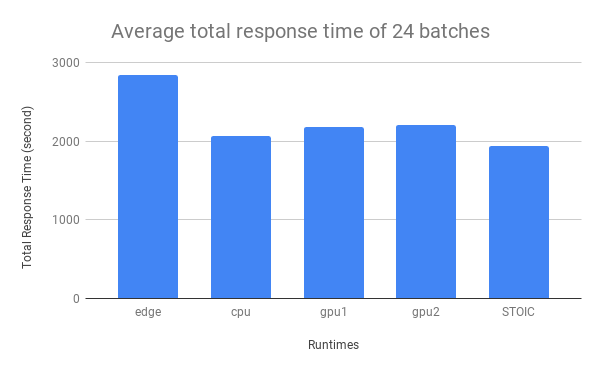
\includegraphics[scale=0.42]{figures/24-batches}
\caption{\textbf{Avg. total response time~($T_r$) on 24-hour dataset}: The x-axis represents runtimes, while y-axis represents the average total response time~($T_r$) by STOIC and four other runtimes on 24-hour dataset. The data labels on columns are specific numbers of $T_r$. The 24-hour batch sizes are generated from the distribution of historical data. 
\label{fig:24-batch}}
\end{figure}

To ensure the validity of outcome, We again run such experiment 10 times for each runtime scenario and report the average value. Figure~\ref{fig:24-batch} demonstrates the average total response time~($T_r$) for STOIC and four individual runtimes. Specifically, STOIC achieves the lowest average latency among four other single runtimes and reduces total response time~($T_r$) by 32.05\% (\textit{edge}), 6.48\% (\textit{cpu}), 11.15\% (\textit{gpu1}) and 12.24\% (\textit{gpu2}) respectively. According to such result, we conclude that STOIC outperforms single-runtime scheduling mechanism on empirical dataset and real-world machine learning application.


\section{Related Work}
\label{sec:relate_work}
As related work, we consider recent advances in both machine learning infrastructure and serverless computing domains. In the former area, much research has extended efforts into designing efficient systems for inference and deployment of machine learning models. As a complement to Tensorflow framework, Tensorflow-serving~\cite{ref:tensorflow-serving} integrates new models and updates versions from training to serving. Though it makes seminal exploration on the multi-tenant model hosting service, Tensorflow-serving does not realize authentic high-performing parallelism to handle concurrent heavy query loads. On that note, Clipper~\cite{ref:clipper} constructs a general-purpose low-latency prediction serving system, which attempts to solve the problem of demanding real-time prediction at the client-side and handling heavy query load at the server-side. It also enables the model composition and online learning to improve accuracy and render more reliable predictions. To explore the multi-pipeline techniques, PRETZEL~\cite{ref:pretzel} casts model-serving as a database problem and applies multi-query optimizations to maximize performance. However, both Clipper and PRETZEL could demand considerable compute resources in caching, batching, adaptive model selection and off-line training to maximize throughput. Therefore, they are not optimized for resource-constraint and heterogeneous IoT devices. To the best of our knowledge, STOIC is the first work to addresses this problem by integrating machine learning applications into a serverless architecture that leverages GPU as additional computational resources for IoT devices. We consider it as a promising and extensible solution for high-throughput and low-latency system for online training and machine learning applications in general. 

 To build up an end-to-end system for practical machine learning applications, we need several other components that bring it to fruition. Seneca~\cite{ref:seneca} fine-tunes hyper-parameters of machine learning models on a general-purpose serverless architecture, namely AWS Lambda~\cite{ref:lambda}. It provides a fast and low-cost method to grid search for the best-performing hyper-parameter set, which is essential in the deployment pipeline of machine learning applications. Velox~\cite{ref:velox} offers a low-latency and scalable solution for complex analytical model-serving, in which it completes a missing piece of personalized prediction serving using Apache Spark~\cite{ref:spark}. For calibrating the performance, McGrath et al.~\cite{ref:serverless} propose an empirical methodology to measure the design and performance of serverless platforms, including latency and auto-scaling capability. All these precursory work completes the serverless ecosystem, particularly for better training, inference and serving machine learning applications.

% An example of a floating figure using the graphicx package.
% Note that \label must occur AFTER (or within) \caption.
% For figures, \caption should occur after the \includegraphics.
% Note that IEEEtran v1.7 and later has special internal code that
% is designed to preserve the operation of \label within \caption
% even when the captionsoff option is in effect. However, because
% of issues like this, it may be the safest practice to 
% \label just after \caption rather than within \caption{}.
%
% Reminder: the "draftcls" or "draftclsnofoot", not "draft", class
% option should be used if it is desired that the figures are to be
% displayed while in draft mode.
%
%\begin{figure}[!t]
%\centering
%\includegraphics[width=2.5in]{myfigure}
% where an .eps filename suffix will be assumed under latex, 
% and a .pdf suffix will be assumed for pdflatex; or what has been declared
% via \DeclareGraphicsExtensions.
%\caption{Simulation Results}
%\label{fig_sim}
%\end{figure}

% Note that IEEE typically puts floats only at the top, even when this
% results in a large percentage of a column being occupied by floats.


% An example of a double column floating figure using two subfigures.
% (The subfig.sty package must be loaded for this to work.)
% The subfigure \label commands are set within each subfloat command, the
% \label for the overall figure must come after \caption.
% \hfil must be used as a separator to get equal spacing.
% The subfigure.sty package works much the same way, except \subfigure is
% used instead of \subfloat.
%
%\begin{figure*}[!t]
%\centerline{\subfloat[Case I]\includegraphics[width=2.5in]{subfigcase1}%
%\label{fig_first_case}}
%\hfil
%\subfloat[Case II]{\includegraphics[width=2.5in]{subfigcase2}%
%\label{fig_second_case}}}
%\caption{Simulation results}
%\label{fig_sim}
%\end{figure*}
%
% Note that often IEEE papers with subfigures do not employ subfigure
% captions (using the optional argument to \subfloat), but instead will
% reference/describe all of them (a), (b), etc., within the main caption.


% An example of a floating table. Note that, for IEEE style tables, the 
% \caption command should come BEFORE the table. Table text will default to
% \footnotesize as IEEE normally uses this smaller font for tables.
% The \label must come after \caption as always.
%
%\begin{table}[!t]
%% increase table row spacing, adjust to taste
%\renewcommand{\arraystretch}{1.3}
% if using array.sty, it might be a good idea to tweak the value of
% \extrarowheight as needed to properly center the text within the cells
%\caption{An Example of a Table}
%\label{table_example}
%\centering
%% Some packages, such as MDW tools, offer better commands for making tables
%% than the plain LaTeX2e tabular which is used here.
%\begin{tabular}{|c||c|}
%\hline
%One & Two\\
%\hline
%Three & Four\\
%\hline
%\end{tabular}
%\end{table}


% Note that IEEE does not put floats in the very first column - or typically
% anywhere on the first page for that matter. Also, in-text middle ("here")
% positioning is not used. Most IEEE journals/conferences use top floats
% exclusively. Note that, LaTeX2e, unlike IEEE journals/conferences, places
% footnotes above bottom floats. This can be corrected via the \fnbelowfloat
% command of the stfloats package.



\section{Conclusion}
\label{sec:conclusion}
In this paper, we propose a framework, called STOIC, for executing machine learning applications in hybrid cloud settings based on serverless architecture. STOIC integrates three components: Edge Controller, Edge Cloud, and Public Cloud. When the scheduler at the edge controller receives a batch of images from open field camera traps, it predicts the total response time for processing the batch based on batch size and historical log data. It then schedules the task to the runtime that it predicts to have the least total response time.  Our STOIC prototype considers four different runtime scenarios. When STOIC schedules the task to the public cloud, the edge cloud deploys a serverless function and then relays the request and payload to the public cloud. STOIC returns the result and metrics to the edge controller when the task completes.

We present the design principles, implementation details, workflow and empirical evaluation on real-world machine learning application for STOIC. Our evaluation demonstrates STOIC is able to intelligently schedule machine learning tasks across hybrid cloud deployments and obtain better performance that using any single deployment option in isolation.  Our speed-up percentages range from 6.48\% to 32.05\% for the application and datasets that we study.

As part of future work, we are developing a feedback control loop to dynamically update the deployment and processing time of STOIC tasks. We plan to also investigate the feasibility of executing model-training tasks using STOIC. Finally, we plan to investigate ways of not having sufficient labeling for image classification tasks and to unify the serverless architecture across all edge and cloud systems within the STOIC system and for the applications that execute using it.

% conference papers do not normally have an appendix

%\section*{Acknowledgments}
%This work is funded in part by NSF (CNS-1703560, OAC-1541215, CCF-1539586,
%CNS-1218808, ACI-1541215) ONR NEEC (N00174-16-C-0020), Huawei
%Corporation, and the California Energy Commission (PON-14-304).
%We also thank the  AWS Cloud Credits for Research program, which enabled us to
%perform this research.

% trigger a \newpage just before the given reference
% number - used to balance the columns on the last page
% adjust value as needed - may need to be readjusted if
% the document is modified later
%\IEEEtriggeratref{8}
% The "triggered" command can be changed if desired:
%\IEEEtriggercmd{\enlargethispage{-5in}}

% references section

% can use a bibliography generated by BibTeX as a .bbl file
% BibTeX documentation can be easily obtained at:
% http://www.ctan.org/tex-archive/biblio/bibtex/contrib/doc/
% The IEEEtran BibTeX style support page is at:
% http://www.michaelshell.org/tex/ieeetran/bibtex/
\bibliographystyle{IEEEtran}
% argument is your BibTeX string definitions and bibliography database(s)
\bibliography{ref}
%
% <OR> manually copy in the resultant .bbl file
% set second argument of \begin to the number of references
% (used to reserve space for the reference number labels box)
% \begin{thebibliography}{1}

% \bibitem{IEEEhowto:kopka}
% H.~Kopka and P.~W. Daly, \emph{A Guide to \LaTeX}, 3rd~ed.\hskip 1em plus
%   0.5em minus 0.4em\relax Harlow, England: Addison-Wesley, 1999.

% \end{thebibliography}



% that's all folks
\end{document}
